
\section{Inference Infrastructure}
\subsection{NVFP4 Inference}\label{sec:nvfp4_inference}
At deployment time, we execute the generator in W4A4 NVFP4, either as a quantized backbone with a separate LoRA branch or as a merged W4A4+LoRA model with fused low-rank kernels. Since AR long-video generation is dominated by repeated linear layers and attention GEMMs, replacing BF16 GEMMs with FP4 GEMMs reduces memory traffic and offers an ideal theoretical throughput speedup of up to $4\times$. We additionally materialize quantized weights and drop BF16 master weights after LoRA wrapping, further reducing resident memory. Unlike post-training quantization (PTQ) methods~\cite{zandieh2025turboquant,li2024svdquant,zhao2024vidit}, our backbone is trained with NVFP4-aware training, which better preserves generation quality under W4A4 inference.

\begin{figure}[t]
\centerline{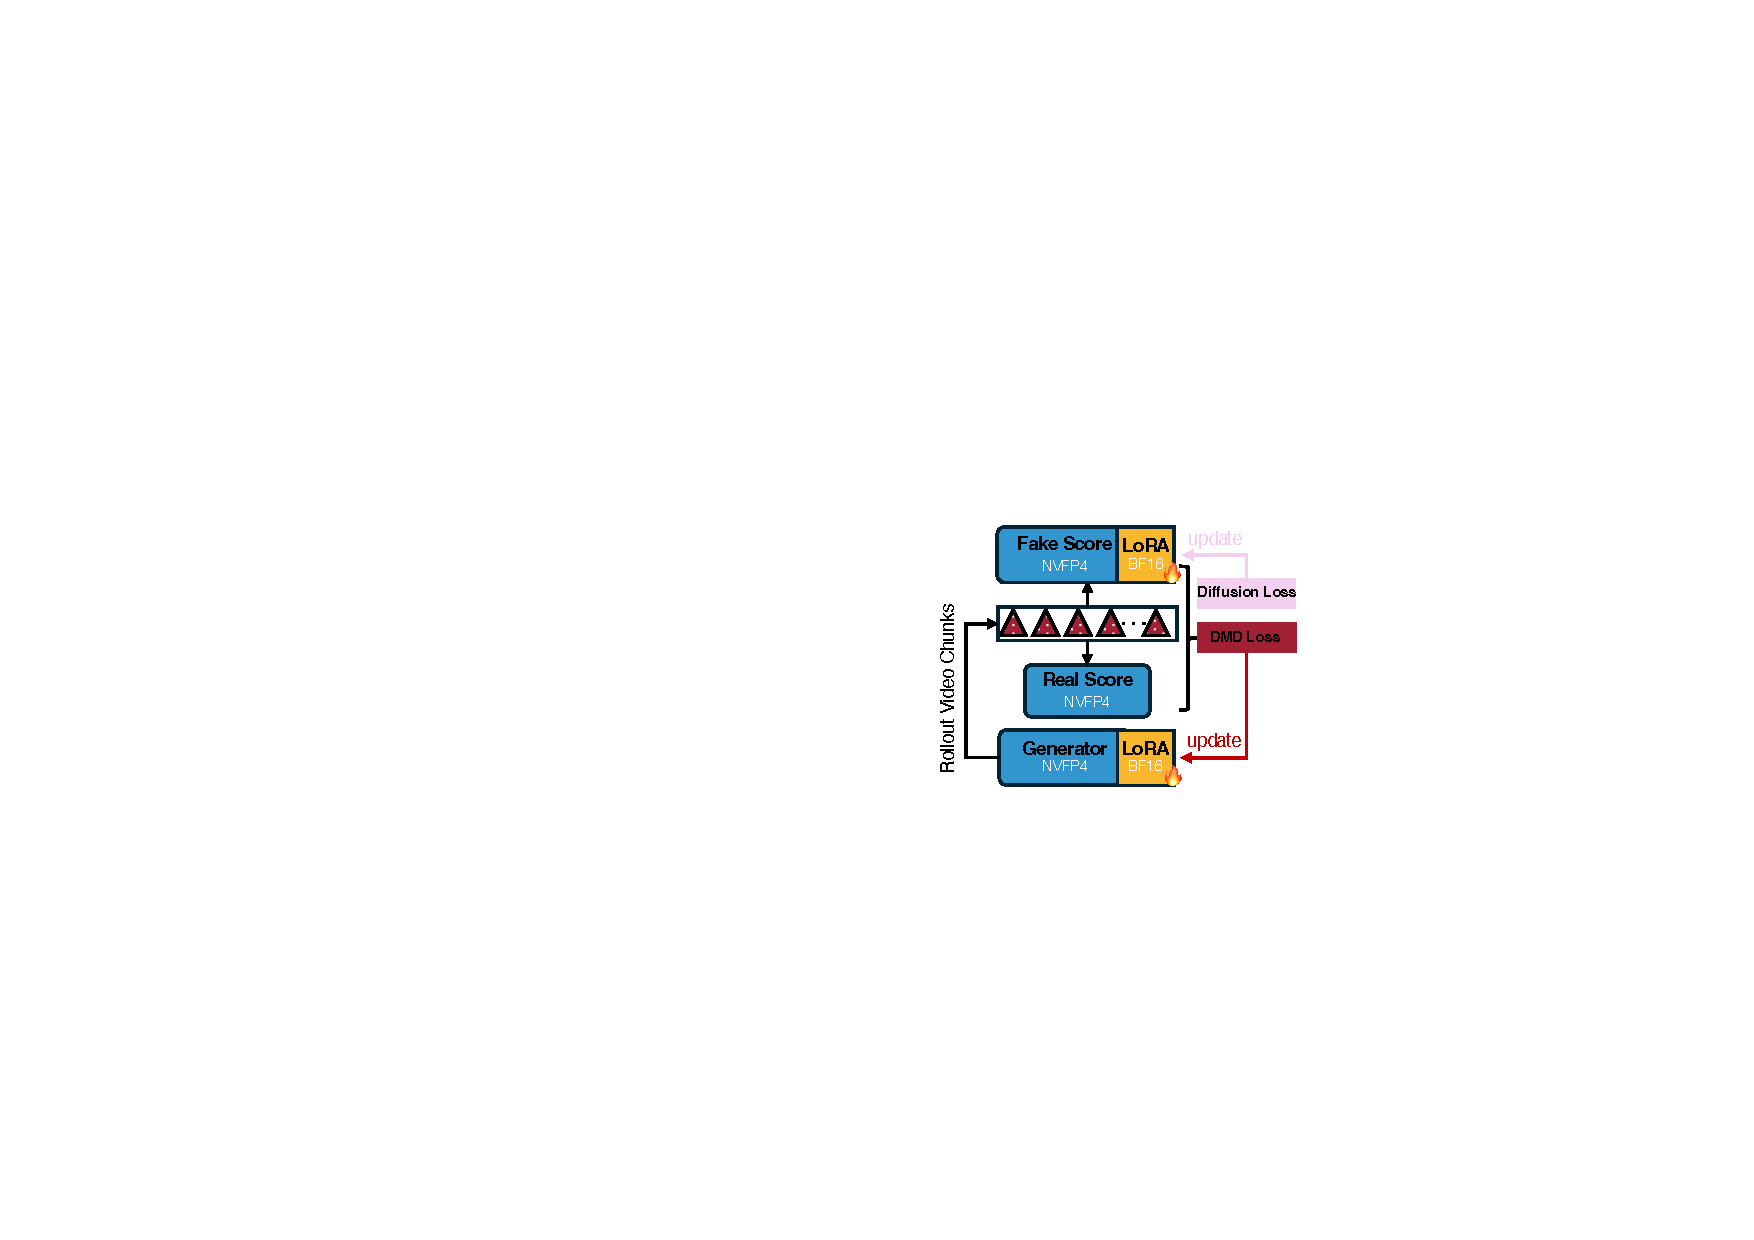
\includegraphics{figs/nvfp4_dmd.pdf}}
\caption{\textbf{NVFP4 DMD training infrastructure.} The generator, real-score model, and fake-score model are colocated under a low-precision NVFP4 setup.}
\label{fig:dmd_training}
\vspace{-10pt}
\end{figure}

\subsection{Parallel KV Quantization}
In AR long video generation, KV cache memory grows linearly with history and quickly becomes a bottleneck~\cite{xi2026quant}. We therefore quantize the cache at the frame-chunk level, aligned with our blockwise pipeline. Each chunk contains $F_c=8$ frames and $T_c = F_c L_f$ latent tokens. For layer $\ell$, the cached KV chunk $c$ is
\begin{equation}
\mathbf{K}_{\ell,c}, \mathbf{V}_{\ell,c} \in \mathbb{R}^{T_c \times H \times d},
\end{equation}
which we reshape to $\mathbb{R}^{(T_c H)\times d}$ and quantize independently with NVFP4 micro-block scaling. For keys, we first apply a simple $K$-smoothing:
\begin{equation}
\bar{\mathbf{K}}_{\ell,c}[t,h,:]
=
\mathbf{K}_{\ell,c}[t,h,:]
- \frac{1}{d}\sum_{u=1}^{d}\mathbf{K}_{\ell,c}[t,h,u].
\end{equation}
We then apply the same adaptive scale selection described in Equation~\ref{eq:4o6}, without repeating the notation here. The storage cost changes from $4 T_c H d \quad \text{bytes}$ to $\frac{9}{8} T_c H d \quad \text{bytes}$, ignoring the amortized tensor-wise scale and padding overhead, which is close to a $3.6\times$ KV-cache compression ratio in practice. This chunkwise NVFP4 cache preserves generation quality while substantially reducing memory footprint. Since LongLive-2.0 uses sink-token sliding windows, each attention step may access multiple cached chunks; we therefore implement a customized parallel CUDA dequantization kernel for efficient in-window reconstruction (Figure~\ref{fig:async_inference}). This keeps the overall KV-cache quantization/dequantization overhead below $2\%$ in practice.

\begin{figure}[t]
\centerline{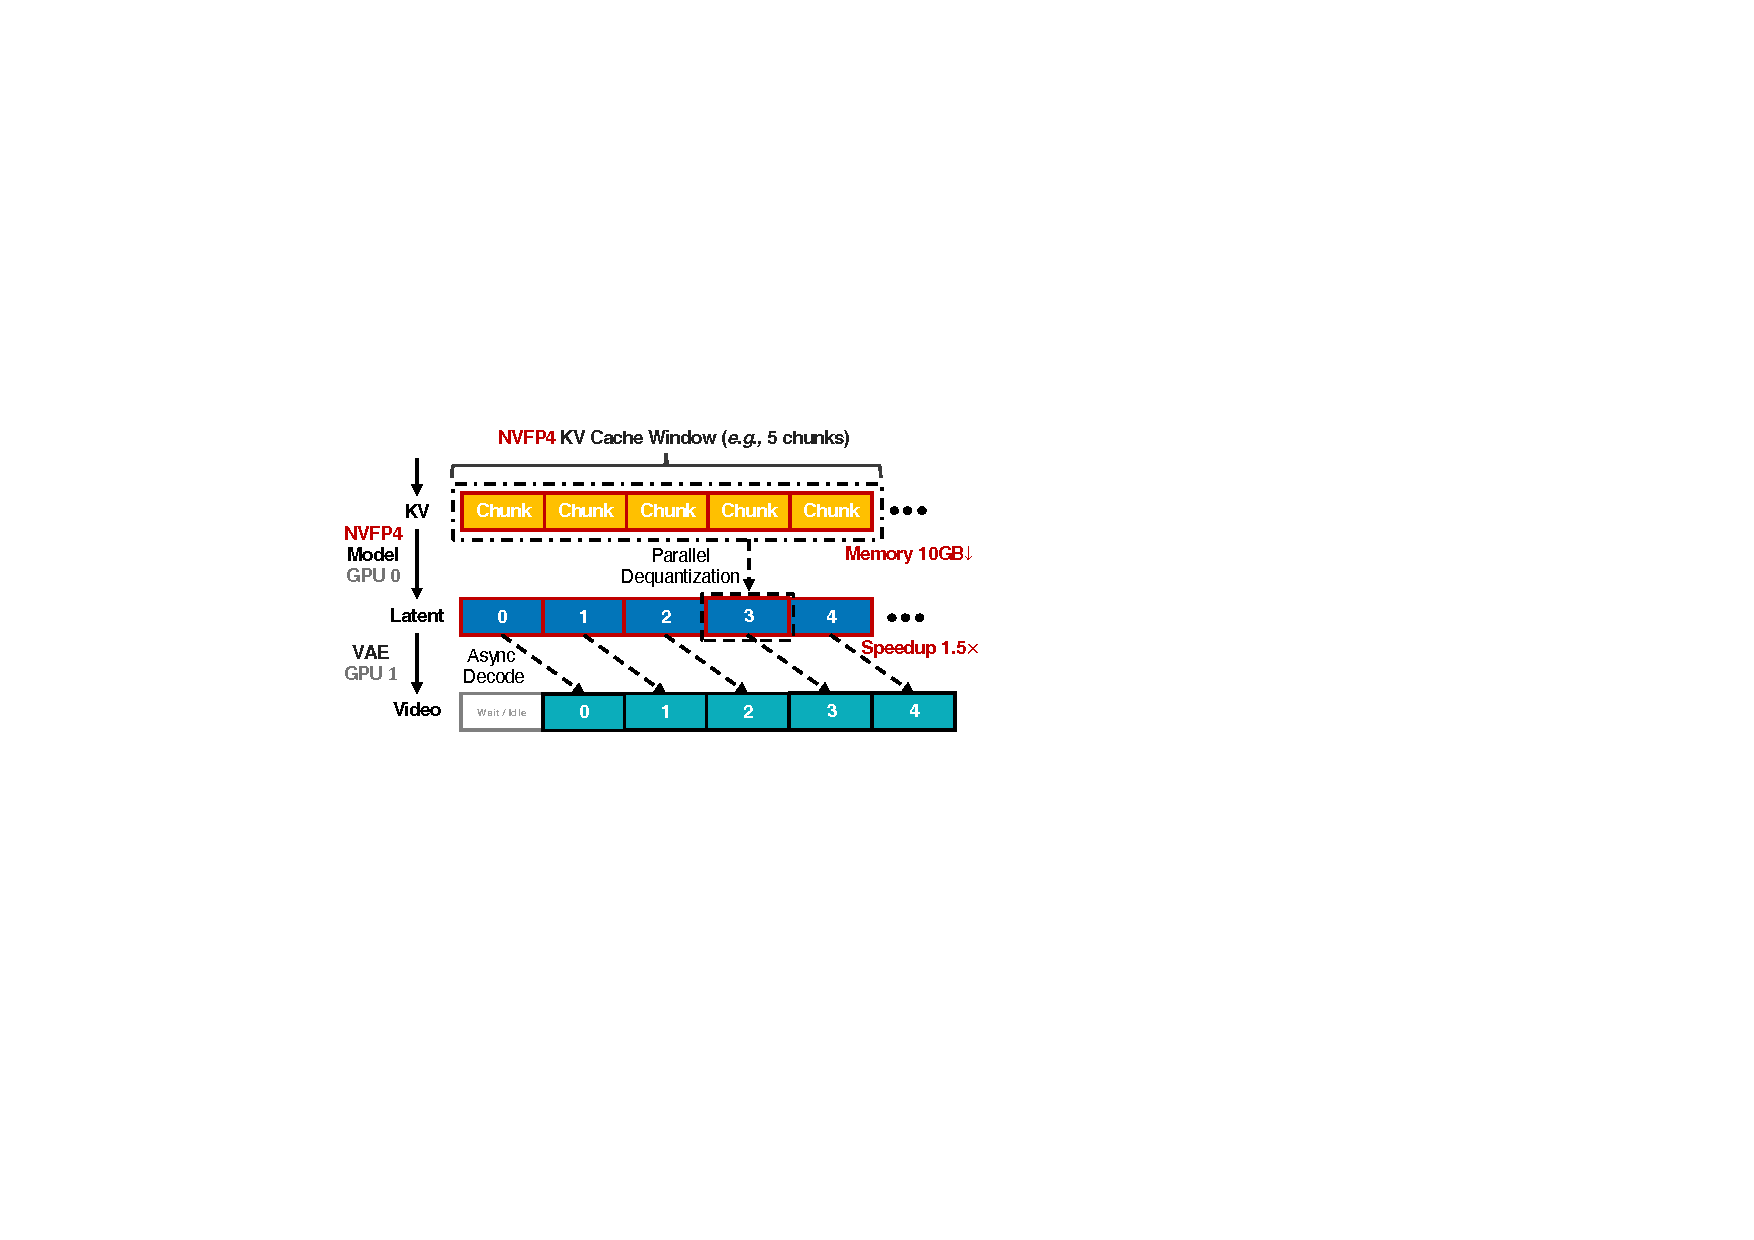
\includegraphics[width=\columnwidth]{figs/inference_all.pdf}}
\caption{\textbf{NVFP4 inference infrastructure.} LongLive-2.0 combines W4A4 NVFP4 inference, quantized KV cache,  and asynchronous VAE decoding to improve throughput and reduce memory for long-video generation.}
\vspace{-10pt}
\label{fig:async_inference}
\end{figure}

\subsection{Asynchronous Streaming Decoding}
The final variational autoencoder (VAE) decoding step is often a major bottleneck in video generation. The centralized decoding scheme used in the baseline LongLive model accumulates all latent chunks before sequential decoding, leading to a VAE-side GPU memory cost of $\mathcal{O}(C \cdot T_c)$ for $C$ chunks and a long end-to-end latency.
We instead design a heterogeneous asynchronous pipeline. We first re-engineer the 3D VAE to support chunk-by-chunk streaming decoding with immediate CPU offloading, reducing the VAE GPU memory footprint to $\mathcal{O}(T_c)$. We then dedicate one GPU to VAE decoding and run it asynchronously alongside the $P$-GPU DiT SP cluster. Let $t_{\text{DiT}}$ and $t_{\text{VAE}}$ denote the per-chunk latencies of denoising and decoding, respectively. 
While the DiT cluster denoises chunk $c+1$, the VAE node decodes chunk $c$. Since the DiT loop is dominant in practice ($t_{\text{DiT}} \ge t_{\text{VAE}}$), decoding is largely hidden behind denoising, reducing the end-to-end latency from $C(t_{\text{DiT}} + t_{\text{VAE}})$ to approximately $C \cdot t_{\text{DiT}} + t_{\text{VAE}}$ and enabling memory-efficient streaming generation.
